\documentclass[11pt,a4paper]{article}
\usepackage[margin=19mm,top=20mm,bottom=20mm]{geometry}
\usepackage{amsmath,amssymb,graphicx,array,fancyhdr,lastpage,textcomp,fancyvrb}
\usepackage{fontspec}
\usepackage[hidelinks]{hyperref}
\setmainfont{texgyreheros-regular.otf}[BoldFont=texgyreheros-bold.otf,ItalicFont=texgyreheros-italic.otf,BoldItalicFont=texgyreheros-bolditalic.otf]
\setmonofont{lmmono10-regular.otf}
\setlength{\parindent}{0pt}\setlength{\parskip}{5pt}
\setlength{\headheight}{14pt}
\pagestyle{fancy}\fancyhf{}
\renewcommand{\headrulewidth}{0.3pt}\renewcommand{\footrulewidth}{0.3pt}
\fancyfoot[L]{\footnotesize by paper.shrit.in\quad |\quad normal}
\fancyfoot[R]{\footnotesize Page \thepage\ of \pageref{LastPage}}
\begin{document}
\fancyhead[L]{\small Digital Systems and Computer Organization}\fancyhead[R]{\small Set A: Ensemble}
{\LARGE\bfseries Worked Solutions}\par{\large Digital Systems and Computer Organization}\par\textbf{Set A: Ensemble | CSE Semester 3}\par
Companion to \texttt{dsco-ensemble.pdf}. Question numbers match that paper. Equivalent correct methods are acceptable. These are independent worked solutions, not an official university marking scheme.\par\medskip\hrule\medskip
Questions 1--5: MCQ answer key, 1 mark each (5 marks total). Questions 6 onward: theory solutions (25 marks total).\par
\noindent\begin{minipage}{\linewidth}\subsection*{1. Signed range}
\textbf{Correct option: (B).} For $n$ bits, the range is $-2^{n-1}$ to $2^{n-1}-1$, giving $-16$ to $15$.
\end{minipage}\par\medskip
\noindent\begin{minipage}{\linewidth}\subsection*{2. Negative representation}
\textbf{Correct option: (D).} Invert \texttt{01001} to get \texttt{10110}, then add 1 to obtain \texttt{10111}.
\end{minipage}\par\medskip
\noindent\begin{minipage}{\linewidth}\subsection*{3. Signed overflow}
\textbf{Correct option: (C).} $11+7=18$ exceeds the maximum signed value 15; the other results lie in range.
\end{minipage}\par\medskip
\noindent\begin{minipage}{\linewidth}\subsection*{4. PLA arrays}
\textbf{Correct option: (A).} A PLA has programmable AND and OR arrays for constructing and combining product terms.
\end{minipage}\par\medskip
\noindent\begin{minipage}{\linewidth}\subsection*{5. Shared product term}
\textbf{Correct option: (B).} $AB$ appears in both outputs and can feed both OR connections.
\end{minipage}\par\medskip
\noindent\begin{minipage}{\linewidth}\subsection*{6. POS minimization and NOR implementation}
Use a K-map with rows AB and columns CD in Gray order 00, 01, 11, 10. X denotes a don't-care.\begin{center}\renewcommand{\arraystretch}{1.2}\begin{tabular}{lllll}\hline AB / CD & 00 & 01 & 11 & 10\\\hline
00 & 0 & 1 & 0 & X\\
01 & 1 & 0 & 1 & 0\\
11 & 1 & X & 1 & X\\
10 & 0 & 1 & 1 & 0\\\hline\end{tabular}\end{center}
Group zeros with useful don't-cares: $\{0,2,8,10\}$, $\{2,6,10,14\}$, $\{2,3\}$ and $\{5,13\}$. These give
\[\boxed{F=(B+D)(\bar C+D)(A+B+\bar C)(\bar B+C+\bar D)}.\]
Each first-level NOR gives the complement of one sum. A final NOR of those four outputs produces their uncomplemented product by De Morgan's law. Generate $\bar B,\bar C,\bar D$ with tied-input NOR gates: $\bar X=\operatorname{NOR}(X,X)$.
\begin{center}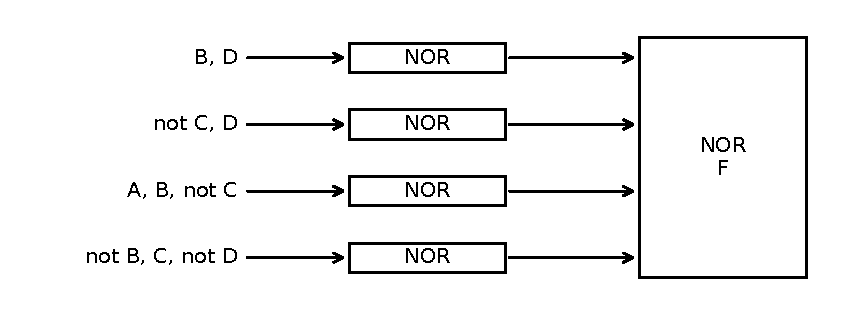
\includegraphics[width=.85\linewidth]{figures/nor-source.pdf}\end{center}
\end{minipage}\par\medskip
\noindent\begin{minipage}{\linewidth}\subsection*{7. Three-bit magnitude comparator}
Define $e_i=a_i\operatorname{XNOR}b_i$. The most significant unequal bit decides the ordering:
\begin{align*}
G&=a_2\bar b_2+e_2a_1\bar b_1+e_2e_1a_0\bar b_0,\\
E_q&=e_2e_1e_0,\\
L&=\bar a_2b_2+e_2\bar a_1b_1+e_2e_1\bar a_0b_0.
\end{align*}
Generate each $e_i$ with an XNOR gate and each complemented input with NOT. The following AND-OR network implements G. Implement L with the same network after exchanging a and b. A three-input AND of the XNOR outputs implements $E_q$. These three networks together form the comparator.\begin{center}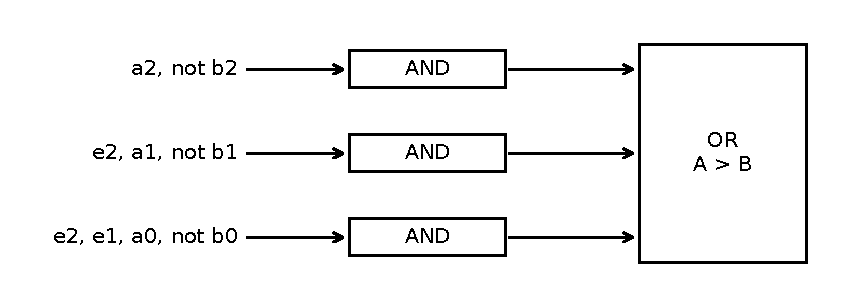
\includegraphics[width=.85\linewidth]{figures/comparator3.pdf}\end{center}
\end{minipage}\par\medskip
\noindent\begin{minipage}{\linewidth}\subsection*{8. Three-input XOR using a multiplexer}
With A and B as select bits (A most significant), $AB=00,01,10,11$ produces $C,\bar C,\bar C,C$, respectively. Thus $\boxed{I_0=C,\ I_1=\bar C,\ I_2=\bar C,\ I_3=C}$. One inverter supplies both complemented-C inputs.\begin{center}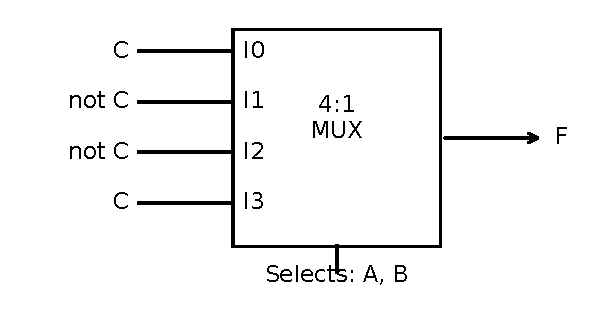
\includegraphics[width=.65\linewidth]{figures/mux.pdf}\end{center}
\end{minipage}\par\medskip
\noindent\begin{minipage}{\linewidth}\subsection*{9. Enabled synchronous up/down counter}
Let A be the most significant state bit and B the least significant. The state table is:\begin{center}\renewcommand{\arraystretch}{1.2}\begin{tabular}{llll}\hline Present AB & E=0, either F & E=1,F=1 & E=1,F=0\\\hline
00 & 00 & 01 & 11\\
01 & 01 & 10 & 00\\
10 & 10 & 11 & 01\\
11 & 11 & 00 & 10\\\hline\end{tabular}\end{center}
A JK flip-flop toggles when $J=K=1$ and holds when $J=K=0$. B toggles whenever enabled. A toggles on an upward carry (B=1,F=1) or downward borrow (B=0,F=0).
\[\boxed{J_B=K_B=E},\qquad
\boxed{J_A=K_A=E(BF+\bar B\bar F)}.\]
Equivalently, the second excitation is E AND (B XNOR F). Connect both flip-flops to the same active clock edge and use the following excitation network.
\begin{center}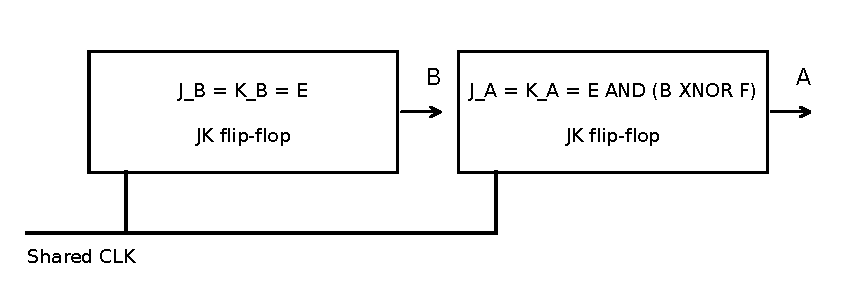
\includegraphics[width=.85\linewidth]{figures/jk-updown.pdf}\end{center}
\end{minipage}\par\medskip
\noindent\begin{minipage}{\linewidth}\subsection*{10. Three-bit synchronous T counter}

For $q_2q_1q_0$, the least significant bit toggles every clock; bit 1 toggles when $q_0=1$; bit 2 toggles when $q_1q_0=11$.
\[\boxed{T_0=1,\quad T_1=q_0,\quad T_2=q_1q_0}.\]
All three T flip-flops use the same clock. Feed $q_1,q_0$ through an AND gate to $T_2$. The sequence is $000,001,010,011,100,101,110,111,000$.
\begin{center}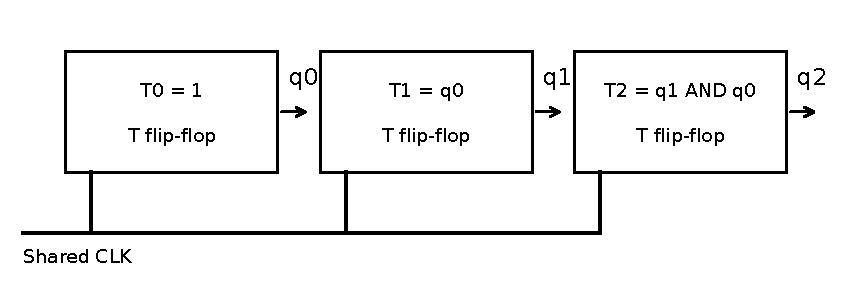
\includegraphics[width=.85\linewidth]{figures/counter3.pdf}\end{center}
\end{minipage}\par\medskip
\noindent\begin{minipage}{\linewidth}\subsection*{11. Four-bit asynchronous ripple counter}
Use four falling-edge-triggered JK flip-flops with J=K=1. Apply the external clock to stage 0 and connect each stage's Q to the next stage's clock, as shown. Clear all stages to 0 before counting.\begin{center}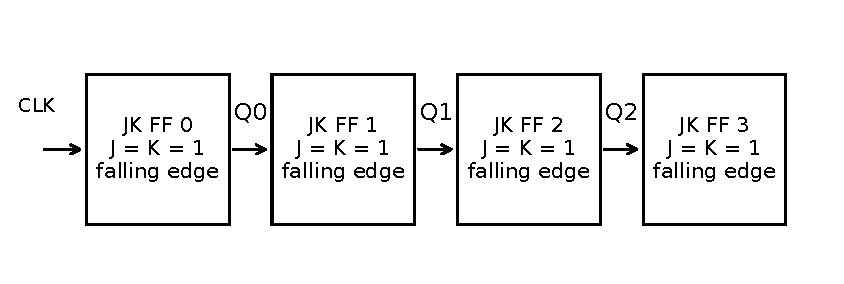
\includegraphics[width=.85\linewidth]{figures/ripple.pdf}\end{center}The output $q_3q_2q_1q_0$ counts 0000 through 1111 and repeats. Output frequencies are $f/2,f/4,f/8,f/16$. Since changes propagate stage by stage, transitions such as 0111 to 1000 pass through intermediate states. Decoding before the ripple settles can produce glitches. The falling-edge convention is necessary for this Q-to-clock up-counter connection.
\end{minipage}\par\medskip
\noindent\begin{minipage}{\linewidth}\subsection*{12. Eight-bit ring counter}
The question leaves reset details open; choose an active-high synchronous reset to load a single 1. This makes the initial state deterministic. Each clock rotates left, including the wrap from bit 7 to bit 0.\VerbatimInput[fontsize=\footnotesize]{code/ring8.v}
The cycle is 00000001, 00000010, 00000100, 00001000, 00010000, 00100000, 01000000, 10000000, then 00000001. Reset must be asserted to enter this one-hot cycle; an all-zero state would otherwise remain zero.
\end{minipage}\par\medskip
\noindent\begin{minipage}{\linewidth}\subsection*{13. Byte and word addressing}
A memory address identifies an addressable unit of storage. An ISA defines how effective addresses are formed and how load/store instructions interpret them. In byte addressing, consecutive addresses select consecutive bytes. A 32-bit word therefore spans four byte addresses, and consecutive aligned words differ by 4. In word addressing, consecutive addresses select entire words, so consecutive words differ by 1. For $2^a$ addressable units, capacity is $2^a$ bytes in the byte-addressed case and $2^a w$ bytes for w-byte word addressing. Word size and address width are separate concepts.
\end{minipage}\par\medskip

\end{document}
